\documentclass[xcolor=table, aspectratio=169, bigger]{beamer}

\usepackage{shyne}

% Theme settings
\setbeamertemplate{navigation symbols}{}

\usetheme{Madrid}
\usefonttheme{structurebold}
\usefonttheme[onlymath]{serif}

\AtBeginSection[]
{ 	\begin{frame}{}

	{
	\usebeamerfont{frametitle}
	\begin{beamercolorbox}
		[wd={\textwidth}, center, sep=.2in, rounded=true, shadow=true]
		{frametitle}
	Week \thesection\\  \secname 
	\end{beamercolorbox}
	}
	
	\end{frame} 
}

\AtBeginSubsection[]
{ 	\begin{frame}{}

	{
	\usebeamerfont{frametitle}
	\begin{beamercolorbox}
		[wd={\textwidth}, center, sep=.2in, rounded=true, shadow=true]
		{frametitle}
	Section \thesection .\thesubsection\\  \subsecname 
	\end{beamercolorbox}
	}
	
	\end{frame} 
}

\title[Week 6]{Stat 201: Statistics I\\ Week 6 }
\author[M. Shyne]{}
\institute[Metro State]{
\includegraphics[width=1.75in]{../images/metro_logo}}
\date[2/25/2019]{
\\ \bigskip \bigskip 
\includegraphics[width=.4in]{../images/cc_big}}



\begin{document}
\frame{\titlepage}

%
% Week 6
%
\setcounter{section}{5}
\section{Binomial and Normal Distributions}

%
% Section 6.1
%
\subsection{Binomial Probability Distributions}

%%%%%%%%%%
\begin{frame}{Binomial distribution}
\begin{block}{}
A \bt{binomial distribution} is a probability distribution representing the number of ``successes" in a fixed number of trials with two possible outcomes.
\begin{itemize}
\pause\item The term ``success" is traditional, but can refer to any outcome of interest.
\end{itemize}
\end{block}
\pause
\begin{exampleblock}{Example}
\begin{itemize}
\item The number of students passing the midterm in class
\begin{itemize}
\item Passing the midterm is a ``success", failing it is a ``failure"
\end{itemize}
\pause\item The number of heads in three coin flips
\begin{itemize}
\item Getting a head is a ``success", getting a tail is a ``failure"
\end{itemize}
\pause\item The number of of car crashes that result in fatalities
\begin{itemize}
\item A fatality is a ``success", no fatalities is a ``failure"
\end{itemize}

\end{itemize}
\end{exampleblock}
\end{frame}

%%%%%%%%%%
\begin{frame}{Requirements for binomial distributions}
\begin{block}{}
There are four requirements to be considered a binomial distribution:
\begin{itemize}
\pause\item The distribution must represent a fixed number of trials
\pause\item Each trial must have exactly two possible outcomes\\(success / failure)
\pause\item Each trial must be independent of the other trials
\pause\item Each trial must have the same probability for success
\end{itemize}
\pause The last two requirements are often summarized as ``independent and identically distributed" and abbreviated as ``iid".
\end{block}
\end{frame}

%%%%%%%%%%
\begin{frame}{Requirements for binomial distributions, example}
\begin{exampleblock}{Example}
Recall the Metro State Statistics Club, with 6 male members and 4 females members. If the three officer positions are selected randomly, does the number of women selected follow a binomial distribution?
\begin{itemize}
\pause\item No. The events are not independent.
\end{itemize}
\end{exampleblock}
\pause
\begin{exampleblock}{Example}
An instuctor is trying a new method of testing students. A test is given once a day for five days, with opportunities to practice and ask questions in between each test. Does the number of times a student passes the test follow a binomial distribution?
\begin{itemize}
\pause\item No. The probability of success changes (hopefully) with each test.
\end{itemize}
\end{exampleblock}

\end{frame}

%%%%%%%%%%
\begin{frame}{Requirements for binomial distributions, example}
\begin{exampleblock}{Example}
Recall the Youth Risk Behavior Survey (YRBS) which found the probability of a teenaged driver had texted or emailed while driving was 0.404. Suppose this is the probability for the population of teenaged drivers. Suppose 30 teenaged drivers are selected at random. Does the number of those drivers that had texted or emailed while driving follow a binomial distribution?
\begin{itemize}
\pause\item Yes. 
\begin{itemize}
\item There is a fixed number of trials (30).
\item Each trial has only two possible outcomes (had or had not texted).
\item Each trial is independent.
\item Each trial has the same probability of ``success."
\end{itemize}
\end{itemize}
\end{exampleblock}

\end{frame}


%%%%%%%%%%
\begin{frame}{Notation for binomial distributions}
\begin{block}{}
\eq{X \sim \f{Binom}(n,p)}
\begin{itemize}
\pause\item The random variable $X$ follows a binomial distribution with $n$ trials and $p$ probability of a success.
\pause\item $q = 1- p =$ the probability of failure
\pause\item $P(X=x)$ is the probability of getting exactly $x$ successes. $x$ must be between 0 and $n$.
\end{itemize}
\end{block}
\pause
\begin{exampleblock}{Example}
The probability a teenaged driver had texted or emailed while driving is 0.404. If the random variable $Y$ is the number of teenaged drivers who had texted or emailed while driving out of a sample of 30,\\ \smallskip
\eq{Y \sim \f{Binom}(30, 0.404)}
\end{exampleblock}
\end{frame}

%%%%%%%%%%
\begin{frame}{Probabilities for binomial distributions}
\begin{block}{}
The formula for binomial probabilities is\\ \smallskip
\eq{ P(X=x) = \binom n x p^x q^{n-x}}
\begin{itemize}
\pause\item $\ds \binom n x$ is read as ``$n$ choose $x$". It is the number of ways to get $x$ successes in $n$ trials. For example, we previously determined that there were three ways to get two heads in three flips, \{ HHT, HTH, THH \}. Thus, $\ds \binom 3 2$ is 3.
\pause\item $p^x q^{n-x}$ is the probability of getting $x$ successes and $n-x$ failures in one particular order.
\end{itemize}
\end{block}
\end{frame}


%%%%%%%%%%
\begin{frame}{Practice: cancer screening}
\begin{block}{}
Recall the cancer screening example. Out of 1000 people screened, the probability of a positive test was 0.1. Suppose a sample 40 of those screened were randomly selected.\\
\medskip
\pause
The random variable $X$ is the number who tested positive in the sample. Does $X$ follow a binomial distribution?
\begin{itemize}
\pause\item Yes. All the requirements are met.
\end{itemize}
\medskip
\pause
What is the notation for $X$?
\begin{itemize}
\pause\item $X \sim \f{Binom}(40, 0.1)$
\end{itemize}
\medskip
\pause
What is the probability that exactly 5 people in the sample tested positive?
\begin{itemize}
\pause\item $P(X=5) = 0.165$
\end{itemize}
\end{block}
\end{frame}


%%%%%%%%%%
\begin{frame}{Parameters for Binomial Distributions}
\begin{block}{}
For $X \sim \f{Binom}(n,p)$,
\begin{itemize}
\pause\item Mean:\\ \smallskip
\eq{ \E(X) = \mu = np }
\pause\item Variance: \\ \smallskip
\eq{\sigma^2 = npq }
\pause\item Standard deviation:\\ \smallskip
\eq{\sigma = \sqrt{\sigma^2} = \sqrt{npq}}
\end{itemize}
\end{block}
\end{frame}

%%%%%%%%%%
\begin{frame}{Parameters, example}
\begin{exampleblock}{Example}
The random variable $Y$ is the number of teenaged drivers who had texted or emailed while driving out of a sample of 30,\\ \smallskip
\eq{Y \sim \f{Binom}(30, 0.404)}

Parameters of $Y$:
\begin{itemize}
\pause\item $\E(Y) = \mu = np = (30)(0.404) = 12.12$
\pause\item $\sigma^2 = npq = (30)(0.404)(1-0.404) = 7.22$
\pause\item $\sigma = \sqrt{\sigma^2} = \sqrt{7.22} = 2.69$
\end{itemize}
\end{exampleblock}
\end{frame}

%%%%%%%%%%
\begin{frame}{Unusual/significant values}
\begin{block}{}
For a given binomial distribution, the boundaries for unusual values can be found. From the range rule of thumb, the lower boundary is $\mu - 2 \sigma$ and the upper boundary is $\mu + 2\sigma$.
\end{block}
\pause
\begin{exampleblock}{Example}
For $Y \sim \f{Binom}(30, 0.404)$, $\mu = 12.12$ and $\sigma = 2.69$. What are the unusual values?
\begin{itemize}
\pause\item The lower bound for unusual values is $\mu - 2 \sigma = 6.74$
\pause\item The upper bound for unusual values is $\mu + 2 \sigma = 17.5$
\pause\item In a random sample of 30 teenaged drivers, it would be unusual to get 6 or fewer, or 18 or more, drivers who had texted or emailed while driving.
\end{itemize}
\end{exampleblock}
\end{frame}

%%%%%%%%%%
\begin{frame}<handout:0>{Group work}
\begin{block}{}
\large
\begin{itemize}
\item Work on question 1, all parts.
\end{itemize}
\end{block}
\end{frame}

%
% Section 6.2
%
\subsection{Normal Distributions}

%%%%%%%%%%
\begin{frame}{Continuous probability distributions}
\begin{block}{}
A \bt{continuous probability distribution} is a description of the probabilities of all possible values of a continuous random variable.
\begin{itemize}
\pause\item Unlike discrete probability distributions, cannot be displayed in a table. There are infinite possible values.
\pause\item Distributions are precisely defined by a probability density function (PDF) or a cumulative density function (CDF).
\pause\item Probabilities of single values are technically always zero, $P(X=x)=0$.
\pause\item Only probabilities of ranges of values have meaning.
\end{itemize}
\end{block}
\end{frame}

%%%%%%%%%%
\begin{frame}{Density curves}
\begin{block}{}
A continuous probability distribution is visualized by a \bt{density curve}, a graph of the probability density function.
\begin{itemize}
\item The total area under the graph is always 1.
\item Probabilities are defined as the area under the curve for the range of values of the random variable.
\end{itemize}
\end{block}
\medskip
{\centering
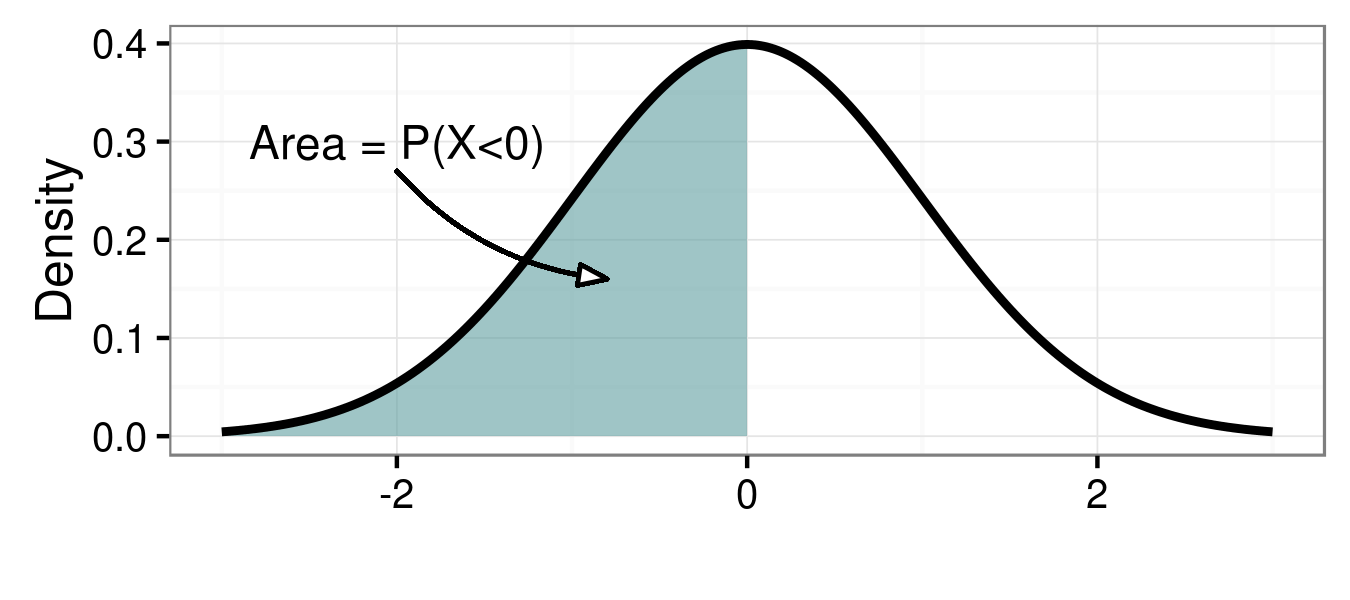
\includegraphics[width=4in]{../images/wk6_density_curve}
\par}
\end{frame}


%%%%%%%%%%
\begin{frame}{Normal distributions}
\begin{block}{}
Recall, normal distributions were defined as having a particular shape.
\begin{itemize}
\item Start with low values, rise to a maximum value, and end with low values.
\item Distribution is symmetric (mirror image) around maximum.
\item ``Bell curve"
\end{itemize}
\end{block}

\pause
\begin{block}{}
Formally, random variable $X$ has a normal distribution with mean $\mu$ and standard deviation $\sigma$...
\begin{itemize}
\item $X \sim N(\mu, \sigma)$
\pause\item PDF: $\ds f(x\mid\mu, \sigma) = \frac 1 {\sqrt{2\pi} \sigma} e^{-\frac{(x-\mu)^2}{2\sigma}}$
\pause\item $\ds P(a <x < b \mid \mu, \sigma) = \frac 1 {\sqrt{2\pi} \sigma} \int_a^b e^{-\frac{(x-\mu)^2}{2\sigma}} \dd x$
\end{itemize}
\end{block}
\end{frame}

%%%%%%%%%%
\begin{frame}{Symmetry of normal distribution}
\begin{block}{}
Normal distributions are perfectly symmetrical, mathematically speaking. That means, the probability a value is greater than some number is equal to the probability of being below the negative of that number.
\begin{itemize}
\item $P(X>c) = P(X < -c)$
\end{itemize}
\end{block}
\smallskip
{\centering
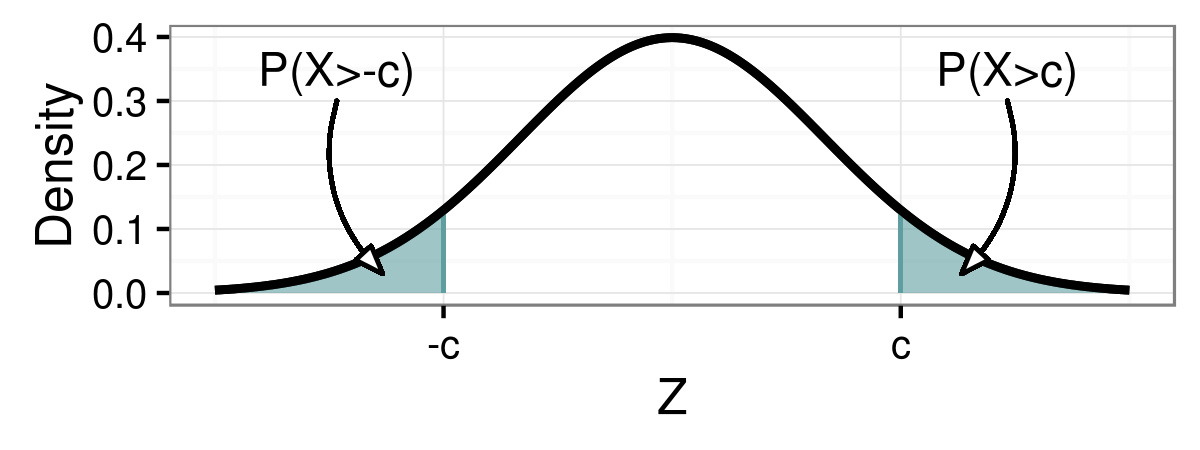
\includegraphics[width=4.5in]{../images/wk6_sym}
\par}

\end{frame}

%%%%%%%%%%
\begin{frame}{Distribution of normal distributions}

\bigskip
{\centering
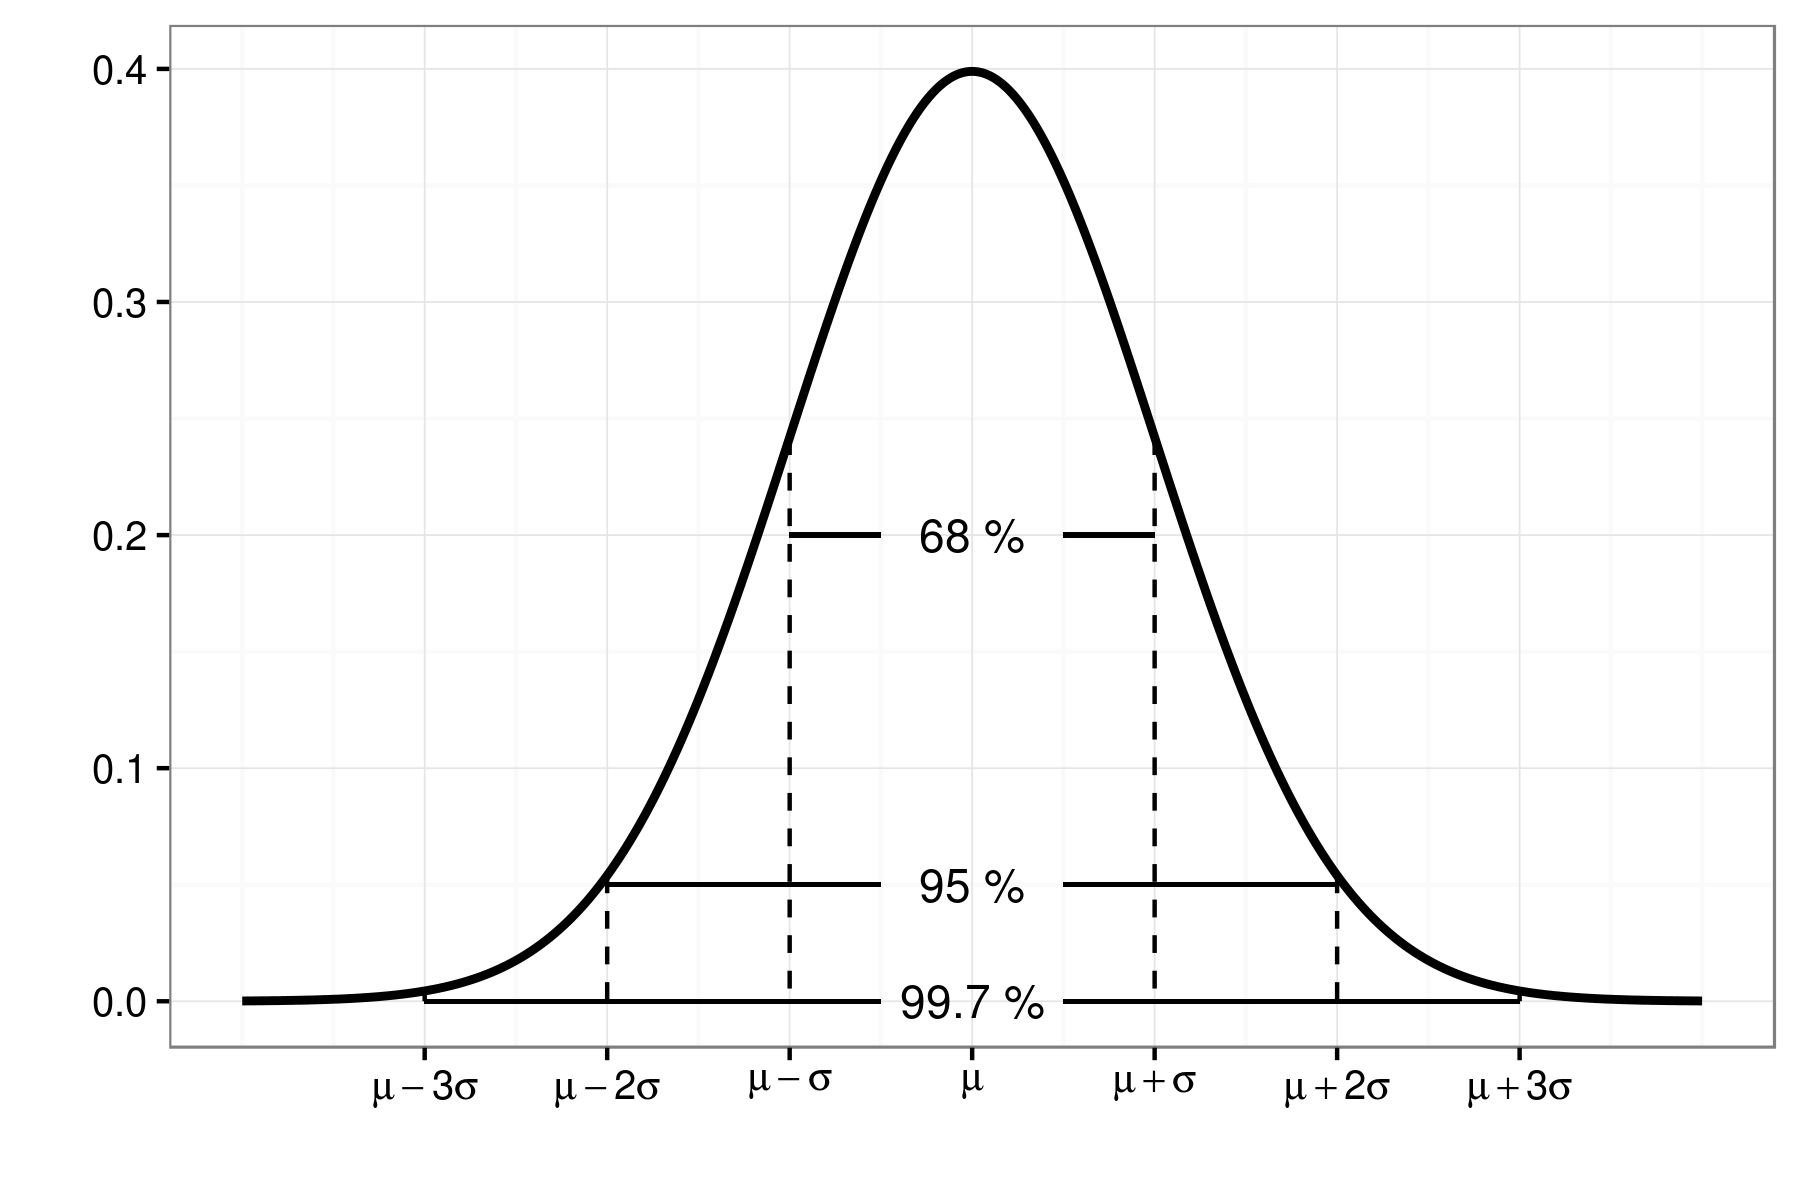
\includegraphics[width=4.25in]{../images/wk06_normal}
\par}

\end{frame}

%%%%%%%%%%
\begin{frame}{Standard normal distribution}
\begin{block}{}
A \bt{standard normal distribution} is a normal distribution with a mean $\mu=0$ and a standard deviation $\sigma =1$. 
\begin{itemize}
\pause\item Also known as the $Z$ distribution.
\pause\item $Z \sim N(0,1)$
\pause\item Values of the standard normal are known as $z$-scores.
\pause\item A $z$-score of 1 ($z=1$) is one standard deviation above the mean, $z=-2$ is two standard deviations below the mean, etc.
\end{itemize}
\end{block}
\end{frame}

%%%%%%%%%%
\begin{frame}{Z distribution}

\bigskip
{\centering
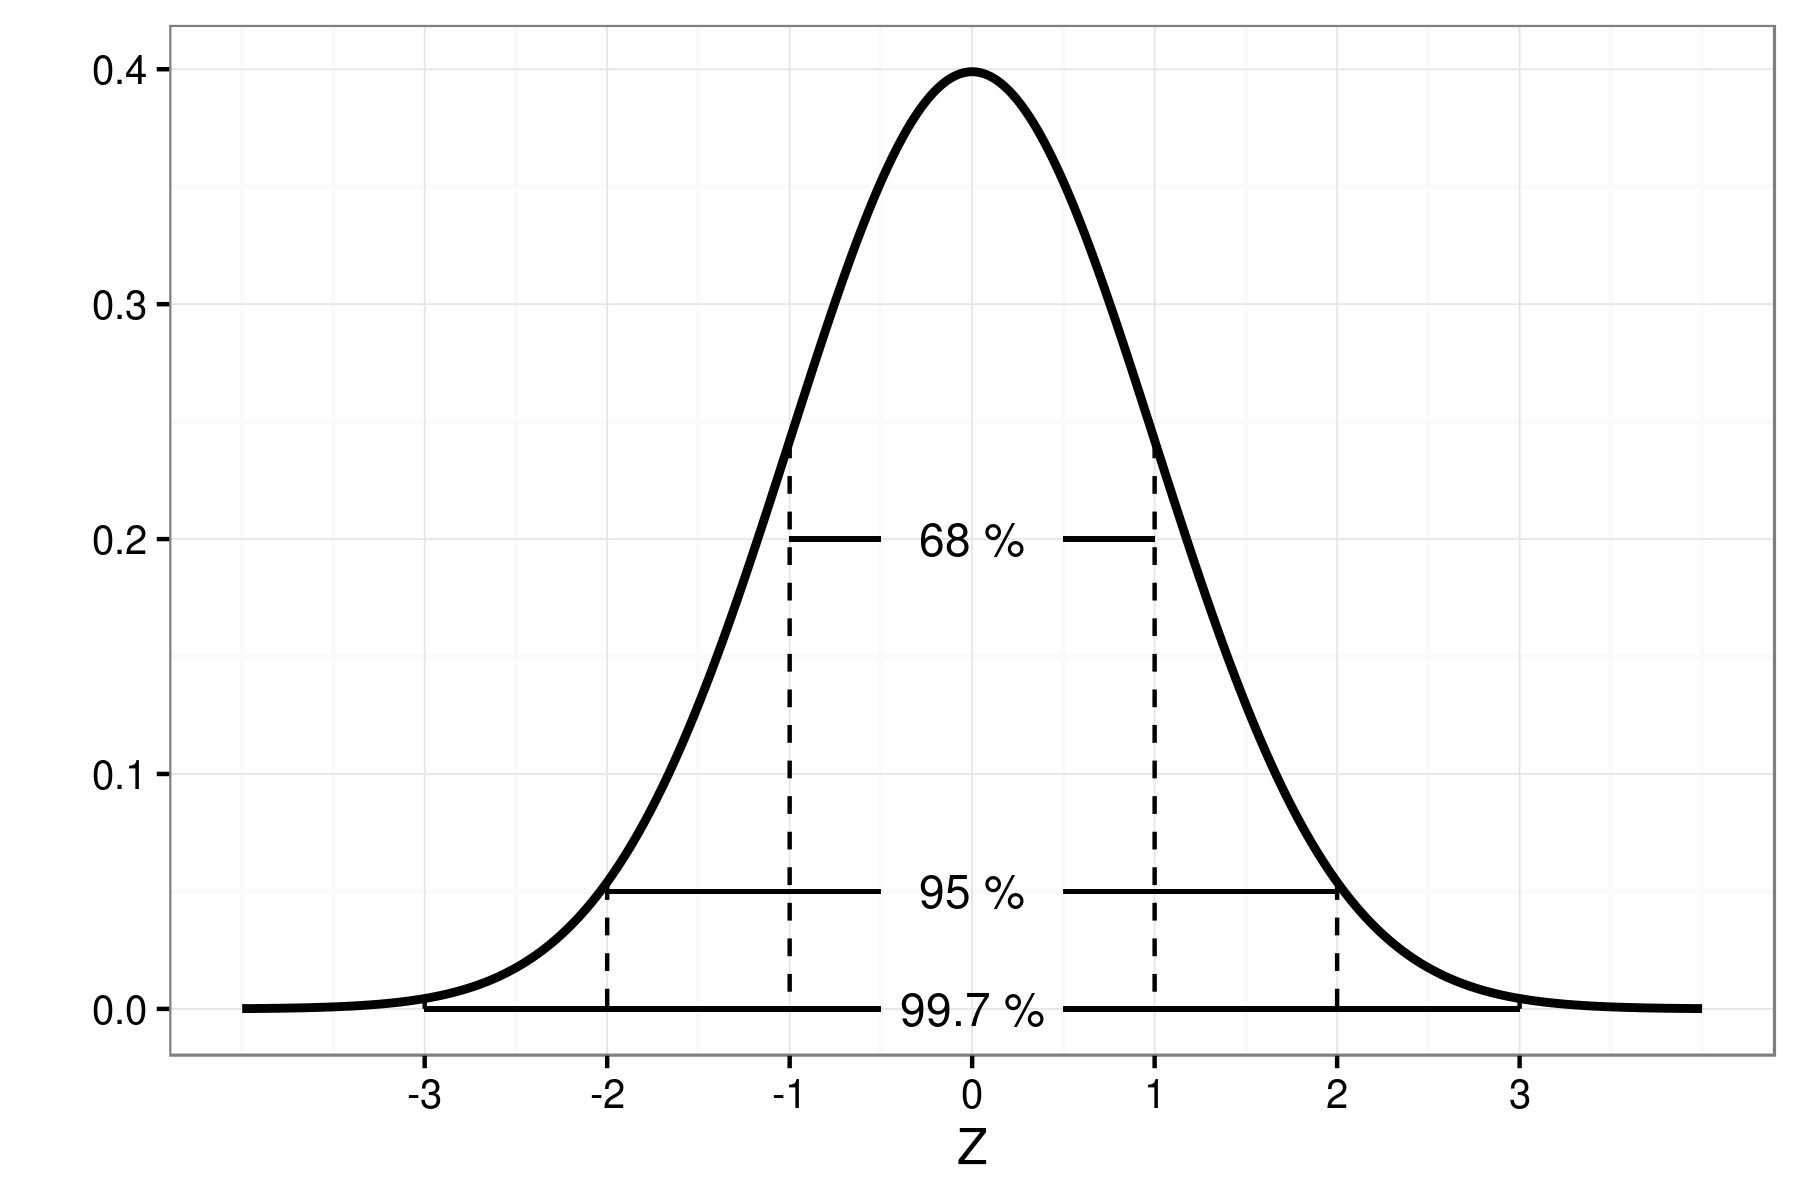
\includegraphics[width=4.25in]{../images/wk06_zdist}
\par}
\end{frame}

%%%%%%%%%%
\begin{frame}{Probabilities of standard normal variables}
\begin{block}{}
Before technological resources, such as computers or statistical calculators, were widely available, tables were used to determine probabilities of events of normal random variables.
\begin{itemize}
\pause\item The table gives the probability for values less than a specified $z$-score, $P(Z < z)$
\pause\item To find probabilities for values greater than a specified $z$-score, subtract table probability from one, $P(Z > z) = 1-P(Z<z)$
\pause\item To find probabilities of ranges of values, subtract lower probability from higher, $P(z_1 < Z < z_2) = P(Z < z_2) - P(Z < z_1)$
\end{itemize}
\medskip
\pause However, using technology is usually quicker and more accurate.
\end{block}
\end{frame}


%%%%%%%%%%
\begin{frame}{Probabilities, example}
\begin{exampleblock}{Example}
Using the standard normal distribution, find the probability a value is less than 0.75 standard deviations above the mean, $P(Z < 0.75)$\\
\smallskip
{\centering
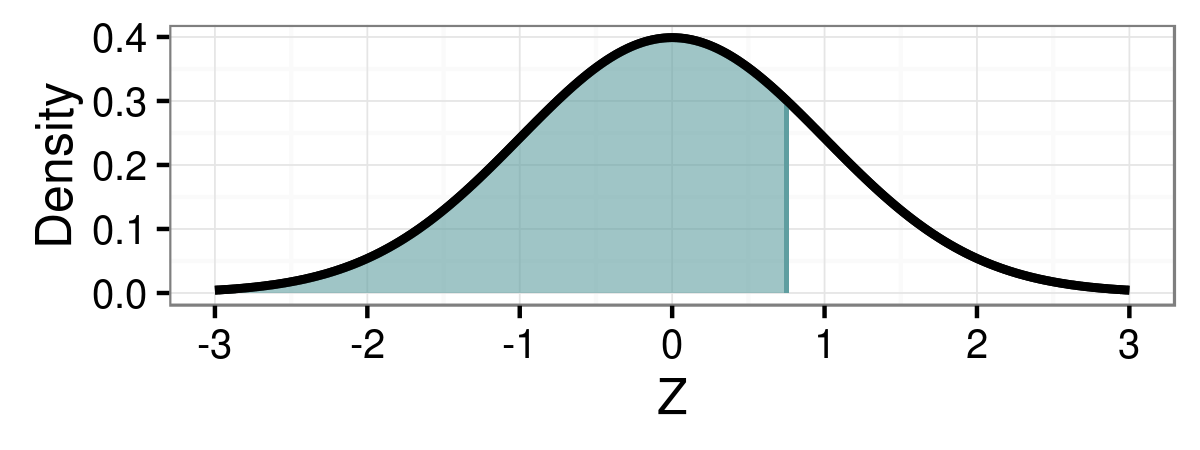
\includegraphics[width=4in]{../images/wk06_ex01}
\par}
\begin{itemize}
\pause\item $P(Z < .75) = \bv{0.773}$
\end{itemize}
\end{exampleblock}
\end{frame}

%%%%%%%%%%
\begin{frame}{Probabilities, example}
\begin{exampleblock}{Example}
Using the standard normal distribution, find the probability a value is greater than 1.3 standard deviations below the mean, $P(Z > -1.3)$\\
\smallskip
{\centering
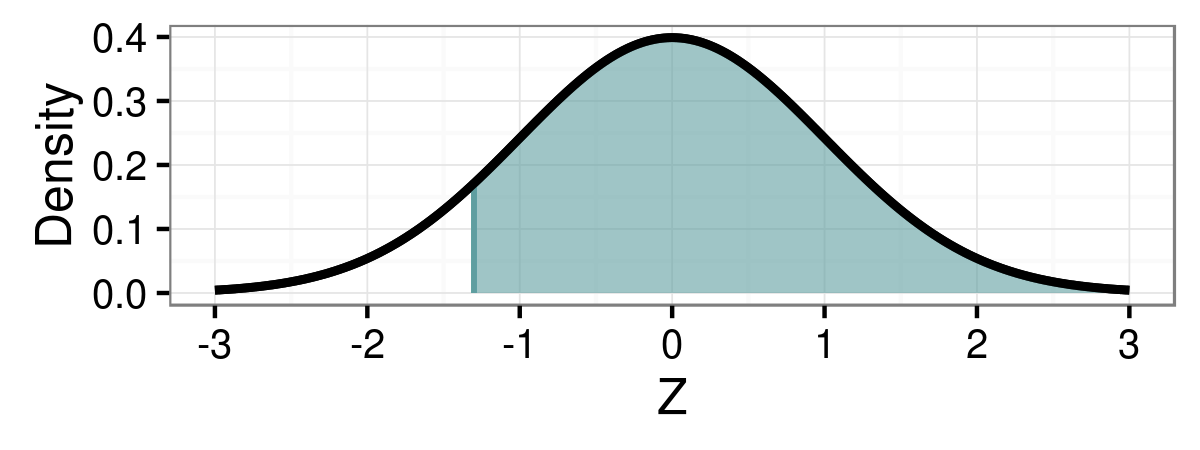
\includegraphics[width=4in]{../images/wk06_ex02}
\par}
\begin{itemize}
\pause\item $P(Z > -1.3) = \bv{0.903}$
\end{itemize}
\end{exampleblock}
\end{frame}

%%%%%%%%%%
\begin{frame}{Probabilities, example}
\begin{exampleblock}{Example}
Using the standard normal distribution, find the probability a value is between -0.2 and 1.1 standard deviations, $P(-0.2 < Z < 1.1)$\\
\smallskip
{\centering
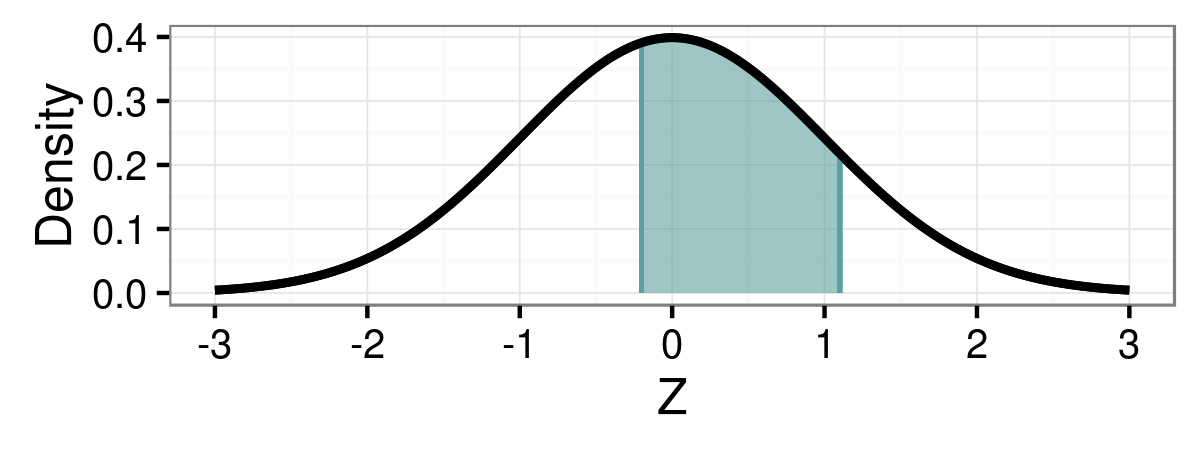
\includegraphics[width=4in]{../images/wk06_ex03}
\par}
\begin{itemize}
\pause\item $P(-0.2 < Z < 1.1) = \bv{0.444}$
\end{itemize}
\end{exampleblock}
\end{frame}

%%%%%%%%%%
\begin{frame}{Finding percentiles}
\begin{block}{}
Often it is desirable to find a $z$-score that is greater than a specified probability, in other words, a percentile. This can be accomplished with the table by locating the desired probability and finding the corresponding $z$-score.\\
\medskip
Again, technology provides an easier and more accurate method.
\end{block}
\end{frame}

%%%%%%%%%%
\begin{frame}{Finding percentiles, example}
\begin{exampleblock}{Example}
What is the z-score greater than 35\% of values? What is $P_{35}$? For what $z$-score is there a 0.35 probability of being less than $P(Z < z) = 0.35$?\\
\smallskip
{\centering
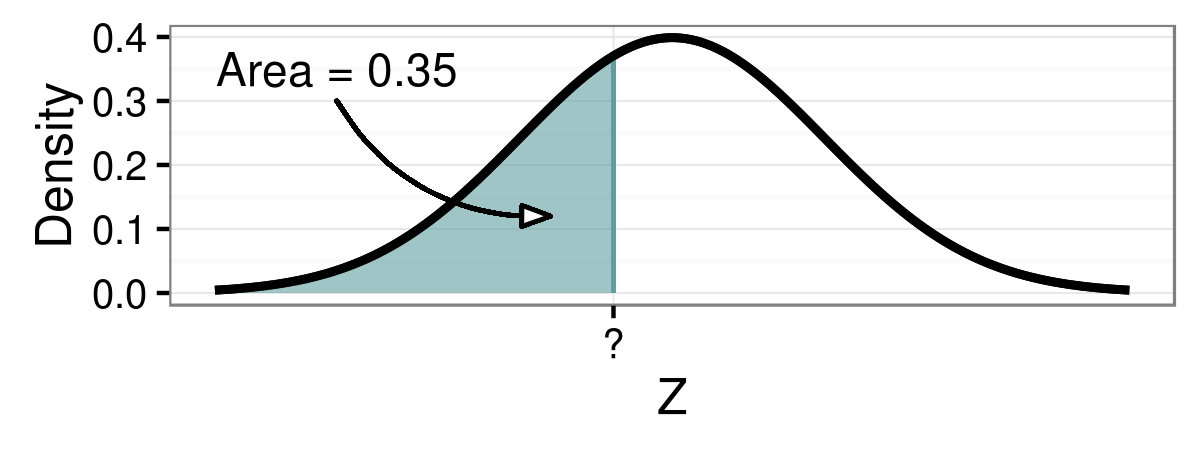
\includegraphics[width=4in]{../images/wk06_ex04}
\par}

\begin{itemize}
\pause\item $P(Z < \bv{-0.385}) = 0.35$
\end{itemize}
\end{exampleblock}
\end{frame}

%%%%%%%%%%
\begin{frame}{Critical values}
\begin{block}{}
In a standard normal distribution, the $z$-score separating usual outcomes from unusual outcomes is known as a \bt{critical value}.
\begin{itemize}
\item The probability denoting unusual events is designated with $\alpha$ (alpha).
\item Then $z_\alpha$ is the critical value such that $P(Z > z_\alpha) = \alpha$
\end{itemize}
\end{block}

\medskip
{\centering
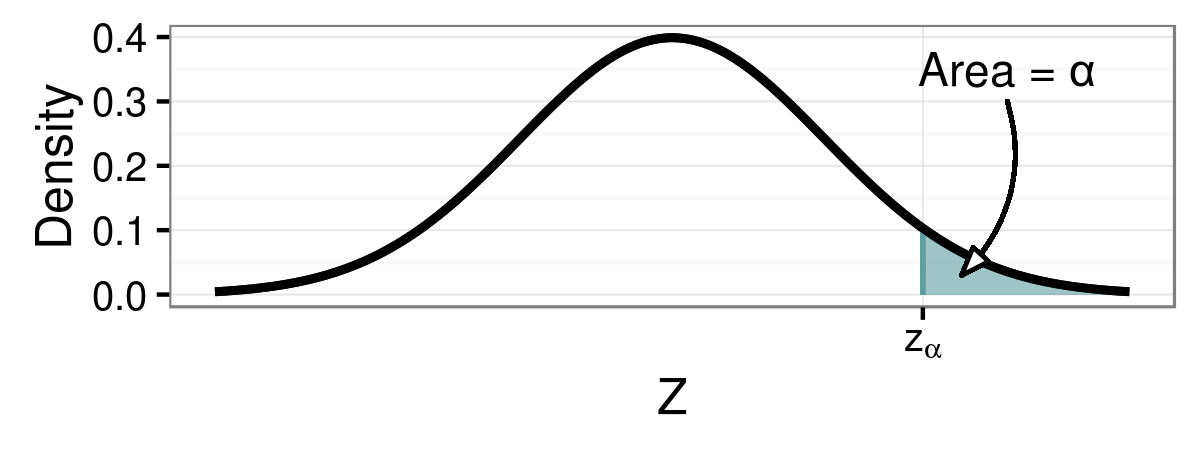
\includegraphics[width=4in]{../images/wk06_alpha}
\par}

\end{frame}

%%%%%%%%%%
\begin{frame}{Critical values, example}
\begin{exampleblock}{Example}
Let $\alpha = 0.05$.\\
\medskip
Find the critical value for $\alpha$. That is, find $z_\alpha$ or $z_{0.05}$.
\begin{itemize}
\pause\item $z_\alpha = 1.645$
\item $P(Z > z_\alpha) = \alpha$ or $P(Z < -z_\alpha) = \alpha$
\end{itemize}
\end{exampleblock}
\smallskip
{\centering
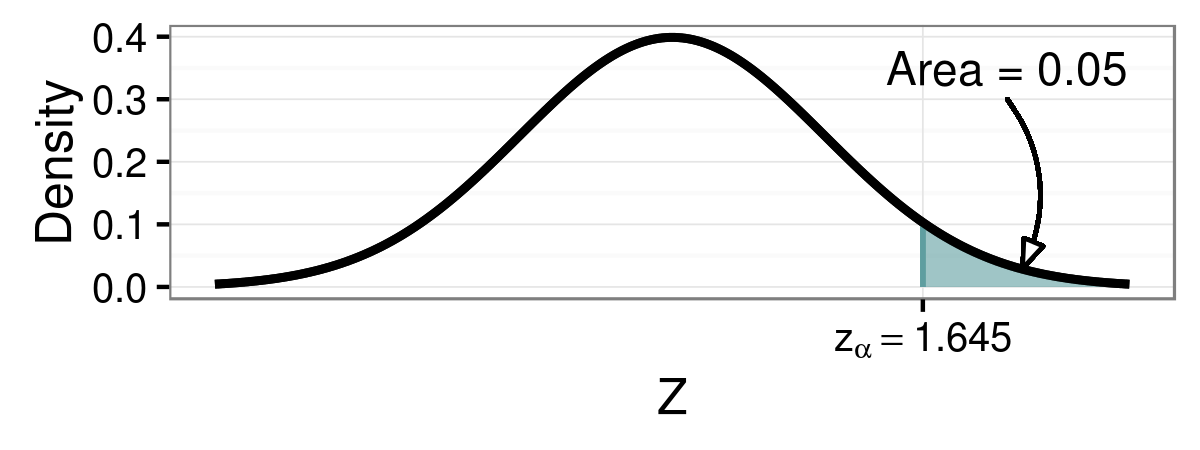
\includegraphics[width=4in]{../images/wk06_crit1}
\par}

\end{frame}


%%%%%%%%%%
\begin{frame}{Critical values, example}
\begin{exampleblock}{Example}
Let $\alpha = 0.05$.\\
\medskip
Find the critical value for $\alpha/2$. That is, find $z_{\alpha/2}$ or $z_{0.025}$.
\begin{itemize}
\pause\item $z_{\alpha/2} = 1.96$
\item $P(Z < -z_{\alpha/2}) + P(Z > z_{\alpha/2}) = \alpha$
\end{itemize}
\end{exampleblock}
\smallskip
{\centering
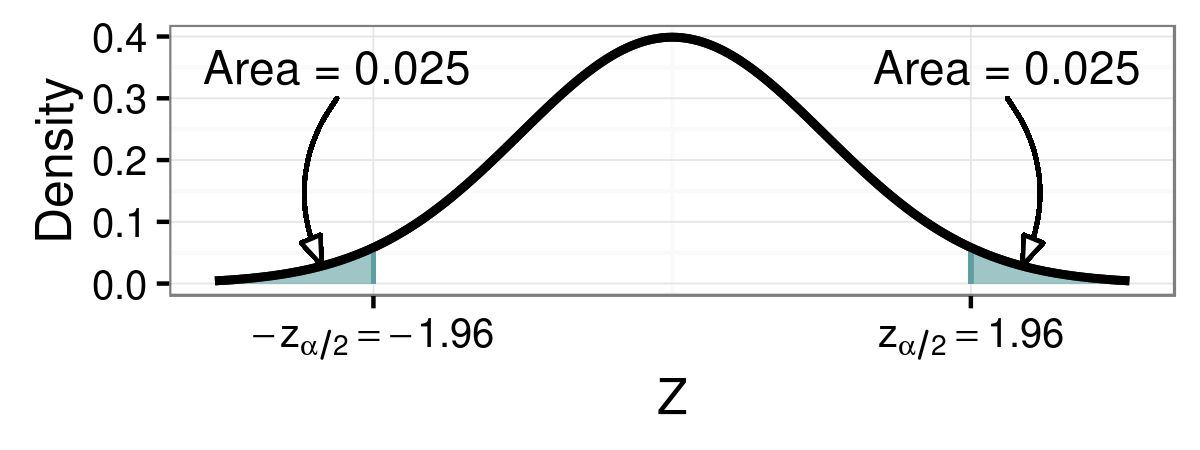
\includegraphics[width=4in]{../images/wk06_crit2}
\par}

\end{frame}


%%%%%%%%%%
\begin{frame}{Non-standard normal distributions}
\begin{block}{}
Non-standard normal distributions, that is normal distributions with a mean other than 0 and/or standard deviation other than 1, are as easy to work with as the standard normal distribution with the help of technology.
\begin{itemize}
\pause\item However, it is still useful to use $z$-scores for comparing values from different distributions.
\pause\item Recall, to convert a value $x$ from a non-standard normal distribution to a $z$-score, and vice versa,\\ \smallskip
\eq{z = \frac {x - \mu}{\sigma} \txtand x = \mu + z\sigma}
\end{itemize}
\end{block}
\end{frame}


%%%%%%%%%%
\begin{frame}{Non-standard normal distributions, example}
\begin{exampleblock}{Example}
An amusement park has made safety their highest priority. They design all their rides to have zero chance of causing serious head trauma, as long as the rider is under 78 inches tall. What proportion of men are in danger at this park?
\begin{itemize}
\pause\item $X_m \sim N(69.2, 5.79)$
\pause\item $P(X_m > 78) = \bv ?$
\pause\item $P(X_m > 78) = \bv{0.064}$
\end{itemize}

\end{exampleblock}
\end{frame}

\begin{frame}{Non-standard normal distributions, example}
\begin{exampleblock}{Example}
The amusement park is designing a new ride. It wants make sure that 85\% of adult women can ride it safely. What is the maximum height the ride should be designed for?
\begin{itemize} 
\pause\item $X_f \sim N(63.7, 5.96)$
\pause\item $P(X_f <  \bv ?) = 0.85$
\pause\item $P(X_f <  \bv{69.88}) = 0.85$
\end{itemize}
\end{exampleblock}
\end{frame}

\begin{frame}{Non-standard normal distributions, example}
\begin{exampleblock}{Example}
The amusement park is growing weary of accommodating the very tall and the very short. It has decided to exclude the most extreme heights among adult men. But it doesn't want to lose to much business, so it will only exclude 5\% of the adult male population. What are the critical values for the tallest and shortest men, for a total of 5\%?
\begin{itemize} 
\pause\item $X_m \sim N(69.2, 5.79), \qquad \alpha = 0.05$
\pause\item $z_{\alpha/2} = z_{0.025} = 1.96$
\pause\item $P(X_m <  \bv{57.85}) = 0.025, \qquad P(X_m >  \bv{80.55}) = 0.025$
\end{itemize}

\end{exampleblock}
\end{frame}

\begin{frame}<handout:0>{Group work}
\begin{block}{}
\large
\begin{itemize}
\item Complete question 2.
\end{itemize}
\end{block}
\end{frame}



\end{document}